\newcommand{\svcourse}{CST Part IA: Introduction to Probability}
\newcommand{\svnumber}{1}
\newcommand{\svvenue}{Churchill, Room TBD}
\newcommand{\svdate}{2022-05-14}
\newcommand{\svtime}{11:00}
\newcommand{\svuploadkey}{PO5ogKIM8KQA22FZS8IAf8gxA8XKi19jxIBVHIfFZ+3GCBXuNUXS9lVN6bNYjxM/}

\newcommand{\svrname}{Mr Matthew Ireland}
\newcommand{\jkfside}{twoside}
\newcommand{\jkfhanded}{right}

\newcommand{\studentname}{Harry Langford}
\newcommand{\studentemail}{hjel2@cam.ac.uk}


\documentclass[10pt,\jkfside,a4paper]{article}
\usepackage{tikz}
\usepackage{float}

% DO NOT add \usepackage commands here.  Place any custom commands
% into your SV work files.  Anything in the template directory is
% likely to be overwritten!

\usepackage{fancyhdr}

\usepackage{lastpage}       % ``n of m'' page numbering
\usepackage{lscape}         % Makes landscape easier

\usepackage{verbatim}       % Verbatim blocks
\usepackage{epsfig}         % Embed encapsulated postscript
\usepackage{array}          % Array environment
\usepackage[nolinks]{qrcode}         % QR codes
\usepackage{enumitem}       % Required by Tom Johnson's exam question header

\usepackage{hhline}         % Horizontal lines in tables
\usepackage{siunitx}        % Correct spacing of units
\usepackage{amsmath}        % American Mathematical Society
\usepackage{amssymb}        % Maths symbols
\usepackage{amsthm}         % Theorems

\usepackage{ifthen}         % Conditional processing in tex

\usepackage[top=3cm,
            bottom=3cm,
            inner=2cm,
            outer=5cm]{geometry}

% PDF metadata + URL formatting
\usepackage[
            pdfauthor={\studentname},
            pdftitle={\svcourse, SV \svnumber},
            pdfsubject={},
            pdfkeywords={9d2547b00aba40b58fa0378774f72ee6},
            pdfproducer={},
            pdfcreator={},
            hidelinks]{hyperref}

\renewcommand{\headrulewidth}{0.4pt}
\renewcommand{\footrulewidth}{0.4pt}
\fancyheadoffset[LO,LE,RO,RE]{0pt}
\fancyfootoffset[LO,LE,RO,RE]{0pt}
\pagestyle{fancy}
\fancyhead{}
\fancyhead[LO,RE]{{\bfseries \studentname}\\\studentemail}
\fancyhead[RO,LE]{{\bfseries \svcourse, SV~\svnumber}\\\svdate\ \svtime, \svvenue}
\fancyfoot{}
\fancyfoot[LO,RE]{For: \svrname}
\fancyfoot[RO,LE]{\today\hspace{1cm}\thepage\ / \pageref{LastPage}}
\fancyfoot[C]{\qrcode[height=0.8cm]{\svuploadkey}}
\setlength{\headheight}{22.55pt}

\ifthenelse{\equal{\jkfside}{oneside}}{

 \ifthenelse{\equal{\jkfhanded}{left}}{
  % 1. Left-handed marker, one-sided printing or e-marking, use oneside and...
  \evensidemargin=\oddsidemargin
  \oddsidemargin=73pt
  \setlength{\marginparwidth}{111pt}
  \setlength{\marginparsep}{-\marginparsep}
  \addtolength{\marginparsep}{-\textwidth}
  \addtolength{\marginparsep}{-\marginparwidth}
 }{
  % 2. Right-handed marker, one-sided printing or e-marking, use oneside.
  \setlength{\marginparwidth}{111pt}
 }

}{
 % 3. Alternating margins, two-sided printing, use twoside.
}

\setlength{\parindent}{0em}
\addtolength{\parskip}{1ex}

% Exam question headings, labels and sensible layout (courtesy of Tom Johnson)
\setlist{parsep=\parskip, listparindent=\parindent}
\newcommand{\examhead}[3]{\section{#1 Paper #2 Question #3}}
\newenvironment{examquestion}[3]{
    \examhead{#1}{#2}{#3}\setlist[enumerate, 1]{label=(\alph*)}\setlist[enumerate, 2]{label=(\roman*)}
    \marginpar{\qrcode{https://www.cl.cam.ac.uk/teaching/exams/pastpapers/y#1p#2q#3.pdf}}
    \marginpar{\footnotesize \url{https://www.cl.cam.ac.uk/teaching/exams/pastpapers/y#1p#2q#3.pdf}}
}{}



\begin{document}

\begin{examquestion}{2007}{4}{1}

\begin{enumerate}[label=(\alph*)]

\item What is meant by a \textit{serialisable} order for two or more
transactions?

A serialisable order $o_s$ for two transactions $T_1$, $T_2$ is an order
containing all operations in both transactions such that there exists a
serial order where all conflicting operations in $o_s$ are ordered in the same
way as in the serial order.

\item Explain how \textit{timestamp ordering} enforces isolation.

Under timestamp ordering, the system decides on a serial order in which each
transaction executes. If any transaction discovers that one of its
conflicting operations is out-of-order then the transaction aborts
(potentially causing cascading aborts). This means that transactions only
commit if the order their conflicting operations took effect in is the same
as some serial order -- the definition of serialisable. Notice that the
converse is not true -- if the system chooses a suboptimal serial order then
some transactions may abort even though there was a valid serial order.

This is implemented by assigning each process a timestamp -- these
timestamps must be globally unique and totally ordered. We must be able to
compare two timestamps and determine which process is first in the serial
order which we are attempting to fulfil. Each shared data has two timestamps
associated with it -- the timestamp of the last transaction to read from it
and the timestamp of the last transaction to write to it. Before any
transaction reads shared data it must check whether any process with a
higher timestamp has written to this data. If so, the transaction cannot
fulfil the serial order and so must abort (potentially causing a cascading
abort).

Before any transaction writes to data, it must check if any transaction with
a higher timestamp has read from the data. If it has, then writing to this
data would be out of order and break isolation. Therefore the transaction
cannot write to data and must abort. If no transaction with a higher ID has
read from the data, the transaction must \textit{then} check whether any
transaction with a higher timestamp has written to the data. If it has then
we return. Notice that we return \textit{if and only if} the data has
been written to after us but was not read by any transactions with timestamps
between the first transaction and the transaction that successfully wrote.
Therefore this does not break isolation. If none of those conditions are
met then the transaction can write to the data.

\item Draw and explain a history graph for two transactions whose invocations
of a set of conflicting operations are serialisable but who are rejected by
TSO .

If TSO assigns $A$ the timestamp 2 and $B$ the timestamp 1 then this
serialisable order will be rejected. As discussed earlier, TSO decides on a
serial ordering when each transaction is issued -- this may not be optimal
and therefore many valid orderings will not be subsets of the serial order
the decided at the start.

$A$ will read from $x$, $B$ will then attempt to write to $x$ but see that
$A$, which has a higher timestamp than $B$ has already read from $x$ and
therefore writing to it could break isolation. Therefore $B$ will abort even
though the order is serialisable.

\begin{center}
\begin{tikzpicture}
\node at (0, 0) {A: 2};
\node at (0, -1) {B: 1};
\draw (0.5, 0) -- (1, 0);
\draw (1, 0.3) rectangle (3, -0.3) node[pos=.5] {Read from $x$};
\draw[-stealth] (3, 0) -- (6.2, 0);
\draw (0.5, -1) -- (3.5, -1);
\draw (3.5, -0.7) rectangle (5.5, -1.3) node[pos=.5] {Write to $x$};
\draw[-stealth] (5.5, -1) -- (6.2, -1);
\draw[-stealth] (2, -0.3) -- (4.5, -0.7);
\end{tikzpicture}
\end{center}

\item Considering Optimistic Concurrency Control (OCC):

\begin{enumerate}[label=(\roman*)]

\item State the properties of a transaction's set of shadow copies that must
be verified at commit time.

\begin{itemize}

\item All versions of data read by the transaction were concurrently correct
at some point in time. The set of times for which all versions of data held
the values read by the transaction is its set of possible start times.

\item There does not exist a committed transaction $T$ which read from any
data the new transaction wishes to write to such that the start time of $T$
is greater than all possible start times for the new transaction.

\end{itemize}

\item Carefully explain the algorithm used by a single-threaded commit-time
validator.

\begin{itemize}

\item Firstly check that both the properties stated above hold.

We can check there exists a time when all data read by the transaction
was concurrently correct by comparing the timestamp associated with the
shadow copy (the last-written timestamp when we read the copy) with the
times the data was written to. If there is a time between when the last data
was read and any were overwritten then this predicate is true. Else it
is false and we must abort/rollback the transaction. Aborting/rollback in
OCC means disregarding the shadow-copies and restarting the transaction.

We then check there does not exist any committed transaction which read from
data we propose writing to that has a timestamp greater than all possible
start times of the new transaction. We do this by checking that for each data
the new transaction is writing to, that the ``last read'' timestamp is
smaller than the last possible start time -- that all data reads are
serialisable. If there is a transaction which is not serialisable then the
new transaction  must abort/rollback. Otherwise we should set the start time
to be the smallest valid start time as this places the least restrictions on
the order.

\item Now we need to commit the data. This can be split into two parts --
writing the data and updating the data's read and write timestamps.

The shadow copies must be swapped in individually atomically to prevent
reads while data structures are in an inconsistent state. We can implement
this by taking out a lock on the data structure while writing to it -- note
there is no ``hold-and-wait'' and so this is fast. Before releasing the lock
we update the list ``last written to'' timestamp to include the timestamp
of the new transaction.

However, if the data has been written to by a transaction with a larger
timestamp then we should not write to it (but should still update the data
with the record that the transaction did). Notice that this is only the case
if the transaction with a larger timestamp never read from the data.

We must then update the list of ``last read'' timestamps associated with the
data that the transaction read.

Since the validator is single-threaded, I assume validating our transaction
cannot be preempted by validating another transaction and therefore assume
validation-validation race conditions are nonexistent.

\end{itemize}

\iffalse

\begin{itemize}

\item Check that both properties above hold.

\item If they do then set the start time to be the smallest start time which
is valid.

\item Then swap the shadow copies in -- they don't have to be atomically since
we assume conflict is rare.

\item Then update the ``last written'' and ``last read'' timestamps
associated with any data the transaction read from or wrote to.

\end{itemize}

\begin{itemize}

\item Check that the reads of the transaction were all valid at some time.
If not then abort.

\item Check that there is no committed transaction with a later start time
which has read from one of the data the transaction is proposing to edit. If
not then abort.

\item Atomically swap the shadow copies (with the updated read/write times)

\end{itemize}

\fi

\end{enumerate}

\item Consider a system in which the transactions cause updates to objects
which are not all located on a single server but which are distributed
widely around the Internet. What factors would influence your choice of
using TSO or OCC to enforce isolation?

\begin{itemize}

\item The rarity of conflicts

OCC aborts only when it is certain there is no serialisable ordering. This
works well under the assumption that conflicts are sufficiently rare that
occasionally doing additional work is more efficient than frequently
aborting safe transactions.

TSO implements a fail-fast mechanism to abort when it is no longer certain
that an order is serialisable. This means that it wastes no work but
frequently aborts transactions which are safe to serialise.

If conficts are common then the underlying assumptions of OCC are broken,
which means OCC will have poor performance. In situations like this, TSO may
be better.

Therefore OCC usually performs better than TSO when conflicts are rare.

\item The proportion of operations which are reads or writes

If there is a high number of reads and a low number of writes then TSO will
frequently abort -- it will attempt to write however transactions with a
lower timestamp will have read from the data we wish to write to and
therefore the transaction will be unsafe and will be forced to abort.
However, in these situations OCC will find a safe serialisation which places
the writes are after the reads.

\item The size of data we operate on

OCC has to make a shadow copy of the data it operates on. If the data that
transactions operate on is large, this may mean that OCC will make copy of
large sections of the database. This is inviable in many situations and
therefore in cases like this, TSO would be preferable.

\item Whether transactions can go idle or fail midway through

Under TSO, transactions can partially complete. If transactions can also
fail or idle they would cause a memory leak or massive cascading abort. In the
first case we assume it will resume at some point and must keep track of all
transactions performed and their inverse operations; while in the second at
some point we assume the transaction has failed and abort all transactions
with higher timestamps or when the transaction resumes and aborts. We may
have to abort thousands of transactions. On a large system this disadvantage
alone makes TSO unusable.

In OCC an idle or failed transaction will not commit. Therefore rest of the
system is unaffected and so there is no problem.

\item The network bandwidth

If the network bandwidth is low then it may be problematic to transfer
enough data for OCC to make shadow copies and swap them back in. This may make
TSO preferable.

\item The network latency

When TSO aborts it has to make a large number of reads and writes to each
server it has communicated with to undo its transactions. This means that on
abort, the transaction has to communicate with every server its read from or
written to. If network latency is high then this may take significant
amounts of time and OCC may be preferable.

\end{itemize}

\end{enumerate}

\end{examquestion}

\begin{examquestion}{2011}{5}{7}

Database concurrency control enables multiple transactions to proceed
simultaneously against a shared database.

\begin{enumerate}[label=(\alph*)]

\item Give an example of \textit{conflicting} and \textit{non-conflicting}
operations on objects in a database.

Conflicting transactions are non-commutative while conflicting operations
are commutative.

An example of a conflicting operation is a read and a write to the same
entry in the database.

An example of a non-conflicting operation is writing to different entries in
the database.

\item Explain how timestamp ordering (TSO) works, and how it responds to
conflicts between transactions.

Under TSO, the server decides on a serial order which it will attempt to
fulfil. Transactions are then assigned a unique, totally ordered timestamp
such that two transactions can compare timestamps and determine which
transaction occurs first in the serial order. The timestamps can be
logical timestamps or timestamps from the system clock.

Data has two labels -- the largest timestamp of any transaction that read
from the data and the largest timestamp transaction that wrote to the data.
This is sufficient to provide safety.

Before a transaction reads from data, it checks to see that no transaction
with a higher timestamp has written to the data -- if so the read would not
match the serial order and therefore cannot take place. So the transaction
would abort; causing all transactions which read from data it had written
to to abort. Notice that if the data has been read by a transaction with a
higher timestamp then the transaction can still read -- reads do not
conflict with other reads.

Before a transaction writes to data it must check both the read and write
timestamps associated with the data. If a transaction with a larger
timestamp has read from the data, then writing to it would be out of the
serial order and is therefore unsafe. So the transaction will abort,
potentially causing a cascading abort. If a transaction with a higher
timestamp has written to the data then the write should return without
writing to the data. This in itself does not break serialisability and
therefore should not cause an abort.

\item Explain cascading aborts and use an example to show how they can
occur with TSO .

Cascading aborts occur when a transaction is forced to abort, however this
transaction has written to data which was then read by other transactions.
This forces these other transactions to abort. This can lead to long chains
of aborts.

Consider the transactions $A$,$B$,$C$ executing concurrently with $V(A) < V(B)
 < V(C)$:
\begin{table}[H]
\centering
\begin{tabular}{c|c|c}
$A$ & $B$ & $C$ \\
\hline
write $\ell_1$ & write $\ell_2$ & \\
			   & 				& read $\ell_1$ \\
read $\ell_2$  & 				&\\
\end{tabular}
\end{table}

When $A$ reads from $\ell_2$, it will abort. However, $A$ wrote to $\ell_1$
and $C$ has read from $\ell_1$ -- therefore $C$ is now incorrect and must be
aborted. So $B$ causes $A$ to abort and $A$ aborting causes $C$ to abort.
This is a cascading abort.

\iffalse

Cascading aborts occur a task which has made writes has to start undoing
operations it has made -- however other tasks had read this updated data and
therefore cannot commit. This means we have to abort a large number of tasks
for a single conflict.

\fi

\item Why is TSO not subject to deadlock?

There are four requirements that a system must meet for it to deadlock:

\begin{itemize}

\item Cyclic Dependency

\item Hold-and-wait

\item No preemption

\item Mutual Exclusion

\end{itemize}

A system will deadlock if and only if it meets all four of these criteria
simultaneously. TSO does not have hold-and-wait -- under TSO if a transaction
is going to read or write then it will either do it immediately after
acquiring the first lock or it will abort. Since TSO cannot meet all
four of the criteria; TSO cannot deadlock.

\iffalse

For a system to Deadlock, four things must happen:

\begin{itemize}

\item Mutual Exclusion

\item Cyclic Dependency

\item Hold and wait

\item No preemption

\end{itemize}

TSO does not hold-and-wait and therefore cannot deadlock.

\fi

\item Explain why TSO distributes well, compared with two-phase locking.

Transactions in TSO do not take out locks meaning transactions never block.
This allows for good concurrency. Two-phase locking takes out locks and
holds them to ensure serialisability -- however often two-phase locking
holds locks longer than is strictly necessary. Therefore two-phase locking
often overly-serialises execution. Two-phase locking is very good at
preventing unnecessary work -- this is important if conflicts are common.
However, as systems scale there become more and more data proportional to
the number of transactions and so the probability of conflicts reduces.
Therefore as systems scale, TSO becomes more effective and 2PL becomes less
effective.

\iffalse

TSO does not take out locks. Two-phase locking takes out locks and
serialises execution on shared data in order to prevent race conditions.

Transactions executing TSO never block and do not take out locks. This means
they never block -- short transactions can execute completely in parallel
without race conditions. This leads to high concurrency.

Conversely, Two-phase locking locks shared data when accessing it. It then
does not release the locks until after it has acquired all the locks it
needs. Two-phase locking is also at risk of deadlock unless locks are
acquired in a partial order. However, acquiring locks in order may
seriously limit concurrency, further limiting performance.

TSO does not lock. This allows better concurrency. Two-phase locking often
ends up locking things unnecessarily and means you can only get good
performance when you operate on a small segment of the system. If you want
to operate on large parts of the system (especially if you only want to
read), then it can be highly inefficient to use two-phase locking. However,
using TSO means you will not take out locks for any longer than strictly
necessary and will significantly better parallelisation.

\fi

\item Construct a workload that performs badly under TSO, and explain why it
does so. What could you do to improve its performance.

The following workload will livelock on a system which does not have any
mitigations:

\begin{itemize}

\item $A$ reads from $\ell_1$, then performs 5s of compute and writes to
$\ell_2$.

\item $B$ does 1s of compute, then reads from $\ell_2$ and immediately
writes to $\ell_1$.

\end{itemize}

The only serialisable order is are one transaction committing before the
other starts. If both transactions start at the same time, they will abort
repeatedly until one commits before the other has started. Since both
processes are long-running, it is unlikely that one will be able to commit
before the other starts -- therefore if both transactions are started at
the same time, they will lead to livelock with high probability.

Assume $B$ starts between 1s before and 4s after $A$ starts -- such that on
the first attempt at execution, $A$ reads $\ell_1$ before $B$ writes to
$\ell_1$ and $B$ reads $\ell_2$ before $A$ writes to $\ell_2$.

Consider both possible timestamp orderings:

\begin{itemize}

\item $V(A) < V(B)$:

$A$ writes to $\ell_1$, then $B$ writes to $\ell_2$ and reads from
$\ell_1$ and terminates. Later, $A$ will read from $\ell_2$ -- however $B$
has written to $\ell_2$ -- so $A$ will abort which causes $B$ to abort and the
cycle restarts.

\item $V(B) < V(A)$:

$A$ writes to $\ell_1$ and $B$ writes to $\ell_2$ (the order of these
operations does not matter) $B$ then reads from $\ell_1$ -- however the
read $\ell_1$ is out of order (as $V(B) < V(A)$ and $A$ has written to
$\ell_1$) and so $B$ will abort and restart.
$A$ has already started, so when $B$ restarts it will be given a timestamp
higher than $V(A)$. Note that this case only happens if $B$ starts before
$A$ does -- therefore when $B$ aborts, there will be at least 4s before $A$
attempts to write to $\ell_1$. This gives $B$ sufficient time to finish
before $A$ attempts to write. This reverts to the case $V(A) < V(B)$.

\end{itemize}

This livelock can only be resolved by allowing one task to commit before the
other task starts.

We could hold a graph of transactions which have aborted and not terminated.
An edge $t_1 \rightarrow t_2$ means that transaction $t_1$ caused $t_2$ to
abort. When a transaction commits, we remove it from this graph. If a
transaction $t$ aborts, we update the graph adding $t$ and attempt to find a
path from $t$ to $t$ (a cycle). If there is a cycle then we remove $t$ from
the graph and do not restart $t$ until at least one transaction in the
cycle finishes. Note that in a cascading abort, we should add transactions
one-by-one to ensure we only remove one transaction from a cycle.

$t$ will only be held back if there is a nontrivial risk of livelock. In
most TSO systems, aborting is rare -- if a transaction does not abort or
cause an abort then its performance will be unaffected by this livelock
detection -- if a transaction aborts once or causes an abort then
the impact on this threads performance will be very small.

\end{enumerate}

\end{examquestion}

\end{document}
